\section{Results}
\label{sec:usage:results}

The specific queries given by the VS and the corresponding oracle labels 
(the oracle, in this case, is the author of this thesis) may be seen in 
Figures~\ref{fig:usage:interesting} and \ref{fig:usage:notinteresting}. Recall 
that the active learner in stage 1 was given a budget of 15 queries. The 
queried plots are not labeled during stage 1 in order to prevent potential bias 
from clouding the user's responses. After stage 2, the user may plot and view 
the corresponding variable names should he/she wish to do so.
 
\begin{figure}[htb]
	\begin{center}
		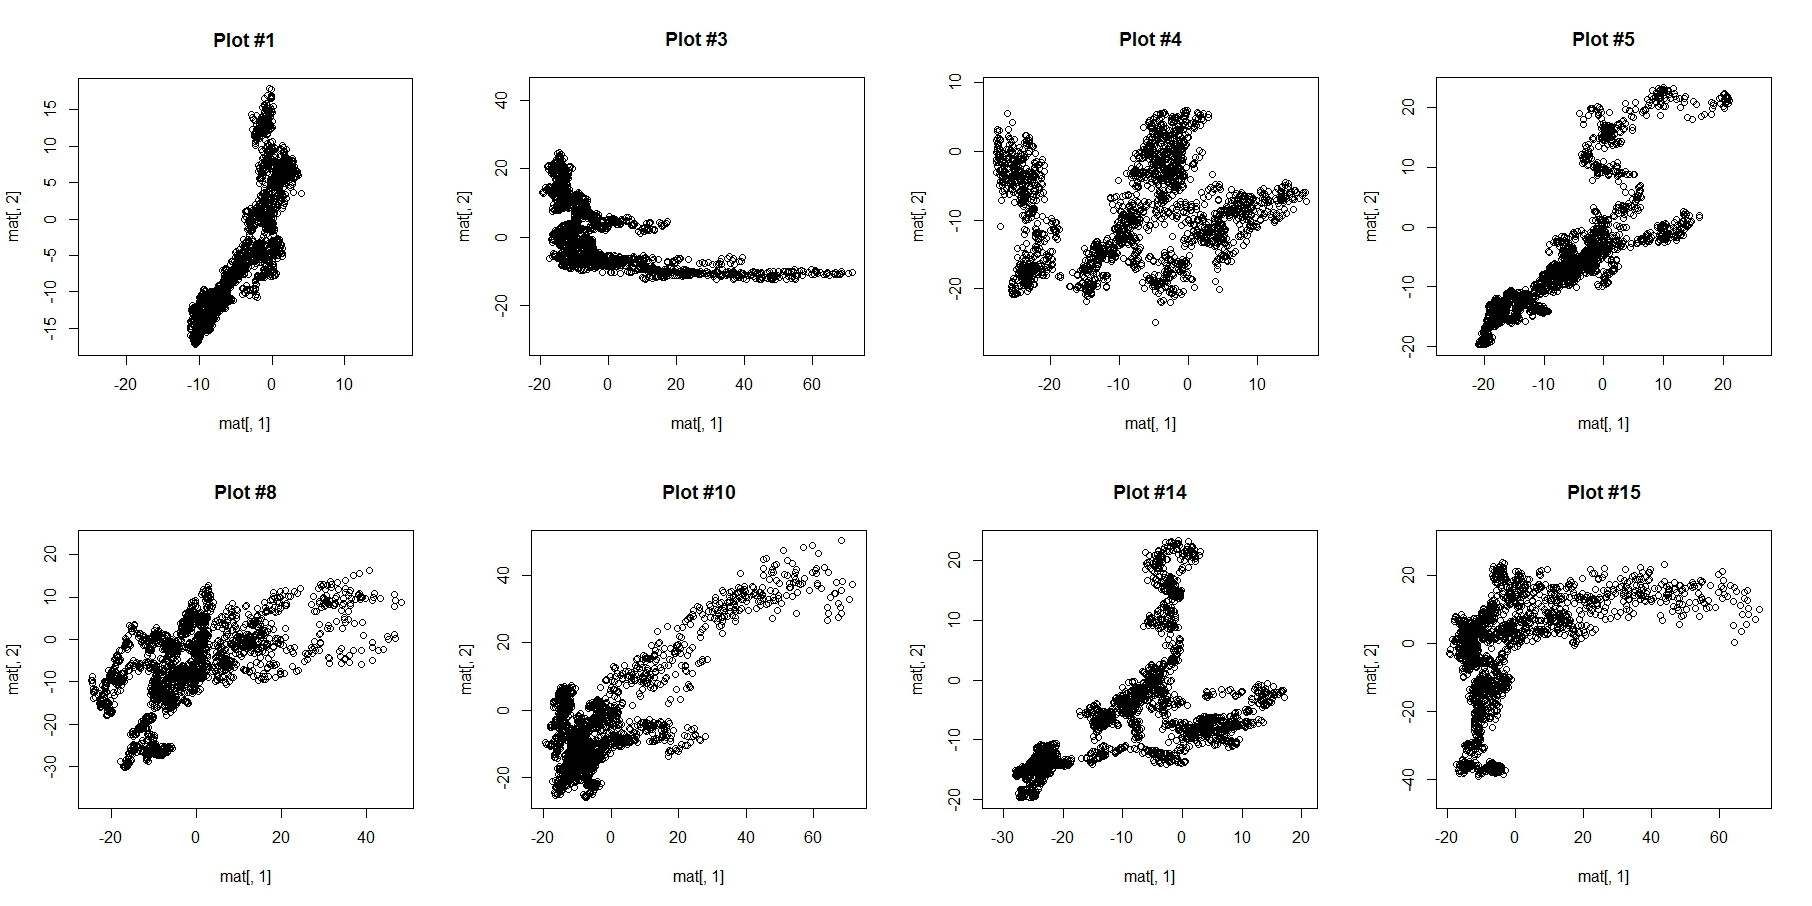
\includegraphics[width=1\linewidth]{ch-usage/figures/y_all}
		\caption[VS queries which were labeled ``visually correlated''.]{VS 
		queries which were labeled ``visually correlated''.}
		\label{fig:usage:interesting}
	\end{center}
\end{figure}

\tablespacing
\begin{figure}[H]
	\begin{center}
		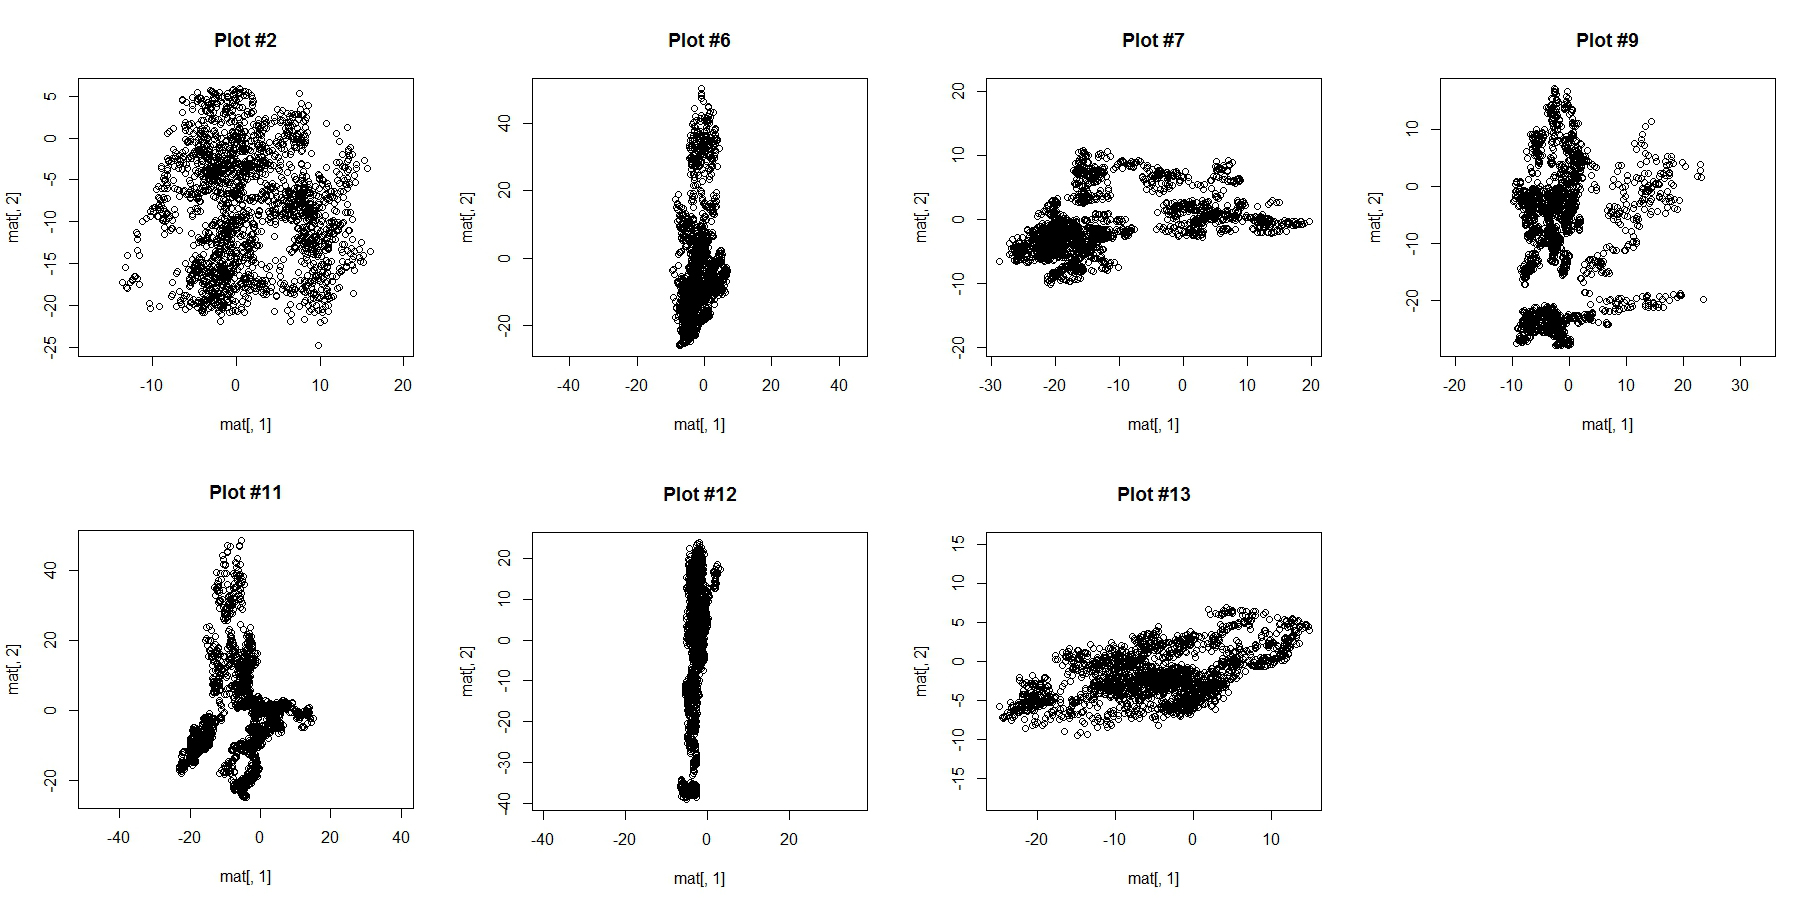
\includegraphics[width=1\linewidth]{ch-usage/figures/n_all}
		\caption[VS queries which were labeled ``not visually correlated''.]{VS 
		queries which were labeled ``not visually correlated''.}
		\label{fig:usage:notinteresting}
	\end{center}
\end{figure}
\bodyspacing

It is also interesting to examine the heat map and association navigator (both 
of which are normalized) in Figure~\ref{fig:usage:heatmaps}, which also 
contains a list of associated criterion. Both maps correspond to the 15 stage 1 
queries. A quick glance at both maps reveal that 
the middle criteria are all zero. It turns out that these criteria 
are associated with various Pearson correlation tests. 
The zero-value heat map entries indicate that the associated $p$-values are all 
extremely low (the correlation is significantly different from zero). In 
particular, this indicates that the criterion 9, 10, 11, 12, 13, and 14 are 
all significant. Consider the actual variable pairs associated with these 
criteria. The first row corresponds to the first queried plot that received a 
label of ``not visually interesting'' (top left plot of 
Figure~\ref{fig:usage:notinteresting}). Specifically, the pair has a Pearson 
correlation coefficient of -0.069 and $p$-value of 0.001728. The Pearson 
correlation coefficient is actually rather close to 0 
(uncorrelated) despite the $p$-value suggesting otherwise. When looking at the 
metric numerically as the heat map and association navigator does, the natural 
response would be to draw an edge as in the $p$-value heuristic given in 
Section~\ref{sec:intro:correlation}. 
However, visually examining the pair's scatter plot (and even just looking at 
the correlation coefficient without the $p$-value) makes it clear that the pair 
is uncorrelated. How did this happen? Because there are 2050 observations of 
each stock, the variance, and subsequently the $p$-value, is low. 
If the correlation graph was constructed solely based on 
the Pearson correlation coefficient $p$-value without consideration of other 
factors, the result would have been less than ideal. This is another scenario 
that demonstrates the usefulness of the VS.

\tablespacing
\begin{figure}[H]
	\begin{center}
		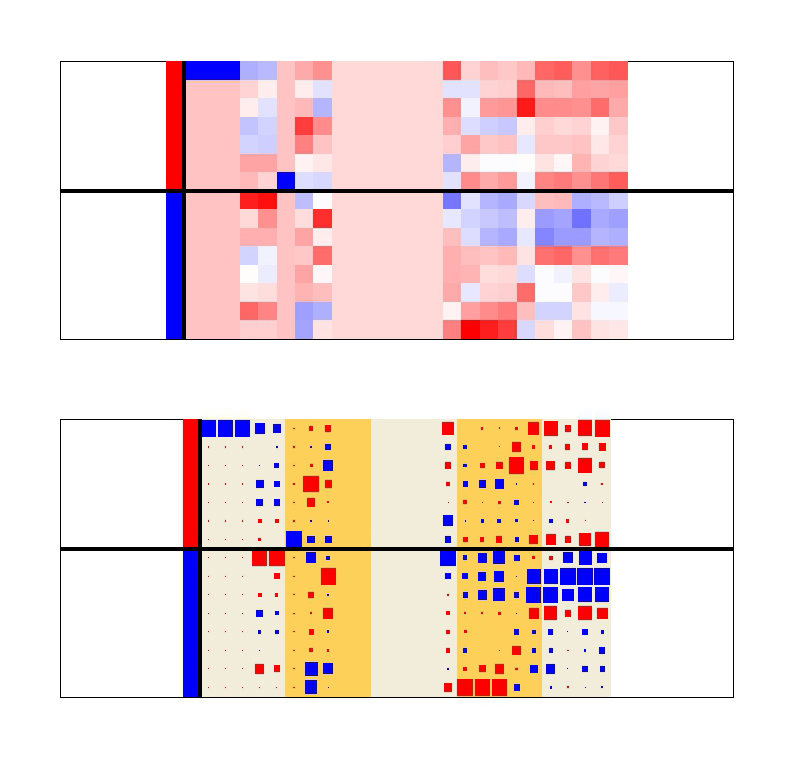
\includegraphics[width=0.8\linewidth]
		{ch-usage/figures/heatmaps}
		\caption[Normalized heat maps of VS queries and user-specified labels.] 
		{\textit{Top:} Standard heat map of the queries and given labels 
		(normalized). 
		\textit{Bottom:} Revised heat map (the association navigator) as 
		proposed by Buja \textit{et al.}~\cite{buja2016} (also normalized). 
		Each row corresponds to a pairwise scatter plot that was queried by the 
		VS and labeled by the user in 
		stage 1. The first column (to the left of the vertical black line) 
		denotes the user's label; as such, there is no size associated with the 
		characteristic. Red indicates ``not visually correlated'' 
		and blue indicates ``visually correlated''. The rest of the columns 
		corresponds to a different criterion of the associated pairwise 
		scatter plot (see Section~\ref{sec:visualizer:scatterplot}). Red 
		indicates a negative value while blue indicate a positive value. 
		Ordered criterion list (left to right, up to down): 
		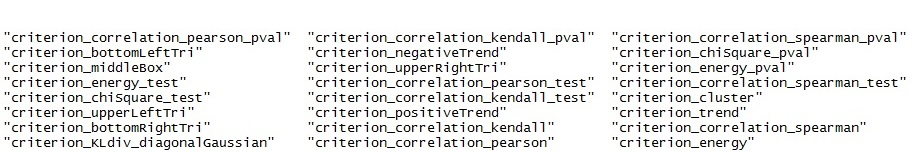
\includegraphics[width=1\linewidth]{ch-usage/figures/criterionlist}}
		\label{fig:usage:heatmaps}
	\end{center}
\end{figure}
\bodyspacing

\newpage
Figure~\ref{fig:usage:hist} is a predicted probability histogram. The 
probability of being ``visually interesting'' or not is computed for 100 random 
pairwise scatter plots. Each probability is computed using the final 
classifier output from stages 1 and 2 of the VS. Most pairs fall within two 
bins (low and high probability). This can be observed as the two hills centered 
near 0.25 and 0.85 in the histogram, indicating that the final classifier is 
quite confident in its labeling of most of the scatter plots.
Figure~\ref{fig:usage:interestingplots} contains the six most ``visually 
correlated'' plots 
selected in the automatic plot generation output of the VS. Most 
plots exhibit a strong positive trend. Interestingly, none of the twelve 
variables (stocks) involved in these six plots ever show up more than once. 

\begin{figure}[htb]
	\begin{center}
		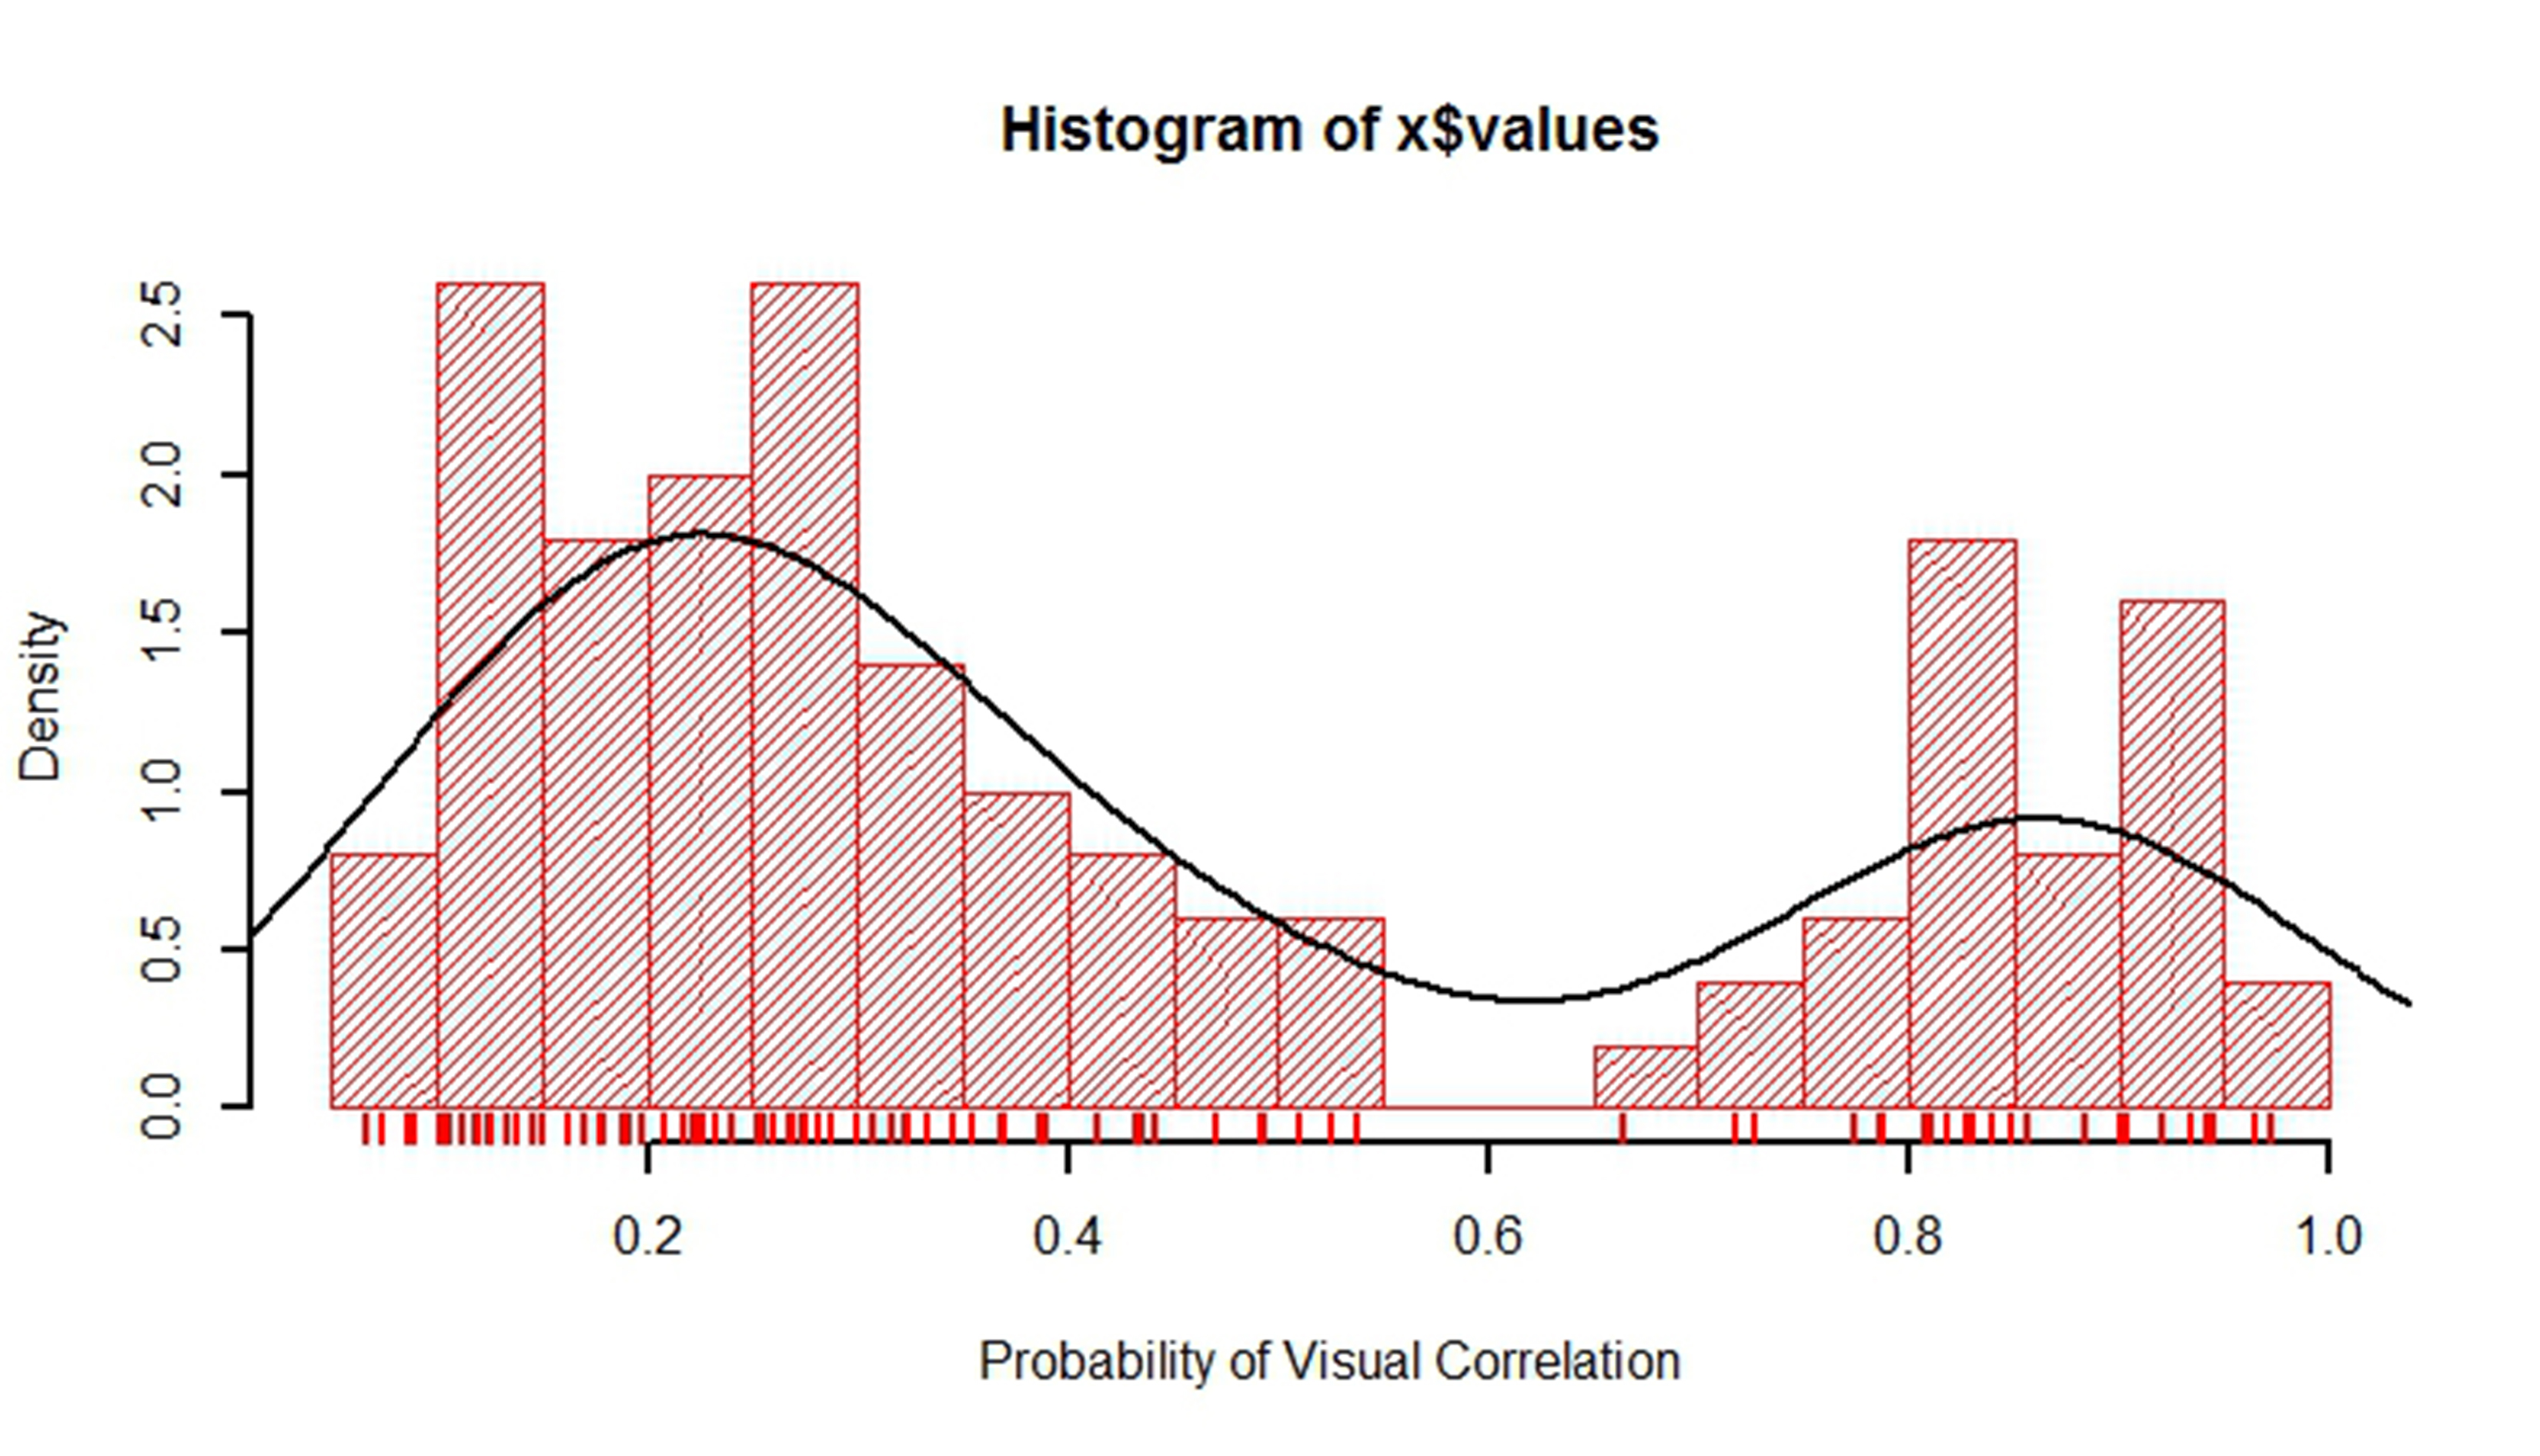
\includegraphics[width=1\linewidth]
		{ch-usage/figures/predicted_probability_histogram}
		\caption[Histogram of predicted probabilities.]{The histogram shows the 
		predicted probabilities for 100 pairwise scatter plots. The 
		probability corresponds to the probability of a plot being 
		``visually correlated'' or ``not visually correlated''.}
		\label{fig:usage:hist}
	\end{center}
\end{figure}

\begin{figure}[htb]
	\begin{center}
		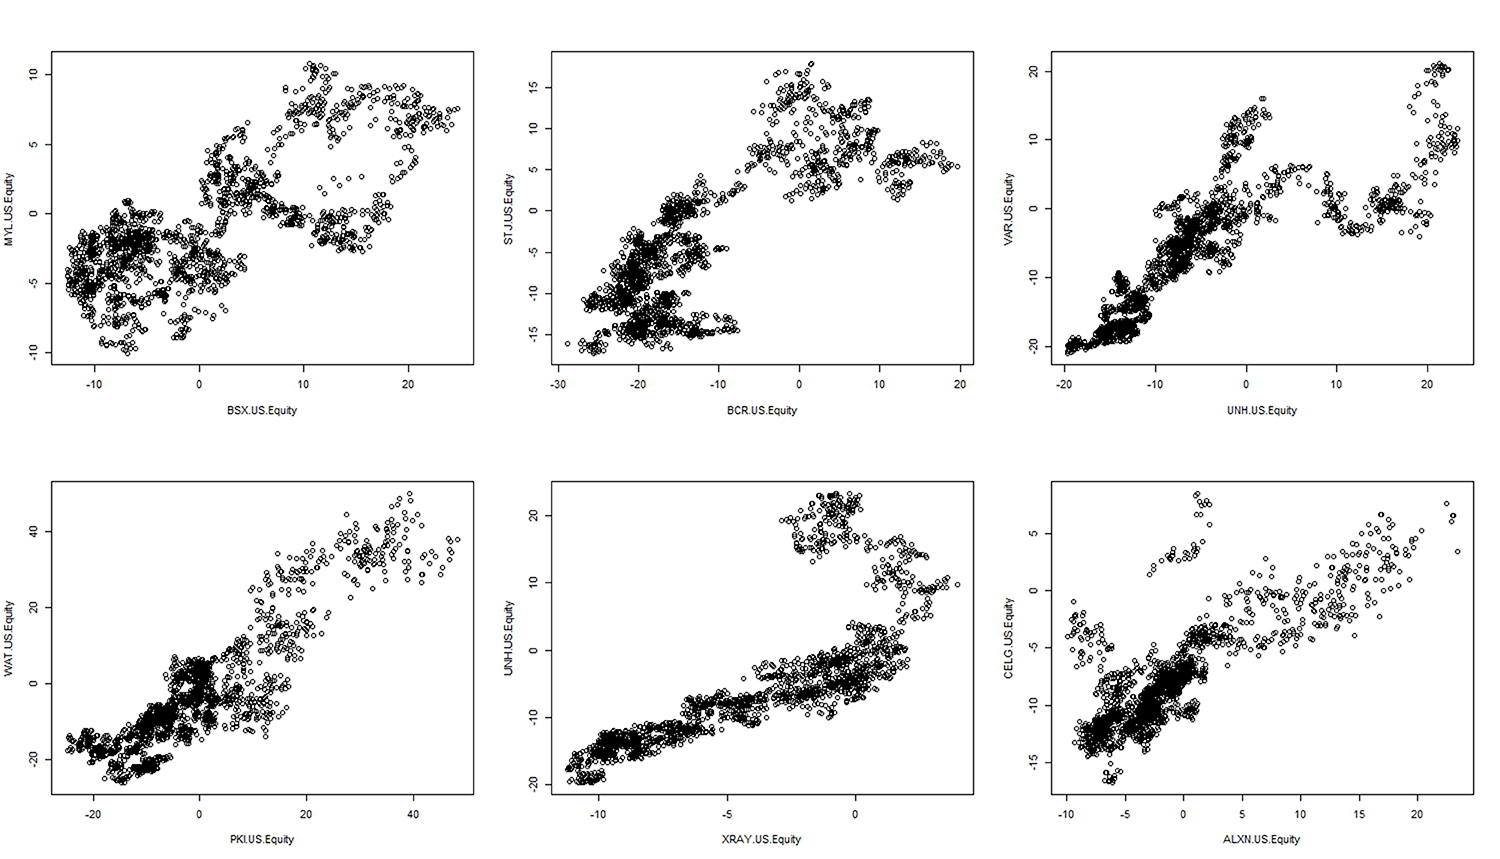
\includegraphics[width=1\linewidth]
		{ch-usage/figures/topinterestingplots}
		\caption[Top six ``visually correlated'' pairwise scatter plots.]{Top 
		six ``visually correlated'' pairwise scatter plots.}
		\label{fig:usage:interestingplots}
	\end{center}
\end{figure}

\tablespacing
\begin{figure}[H]
	\begin{center}
		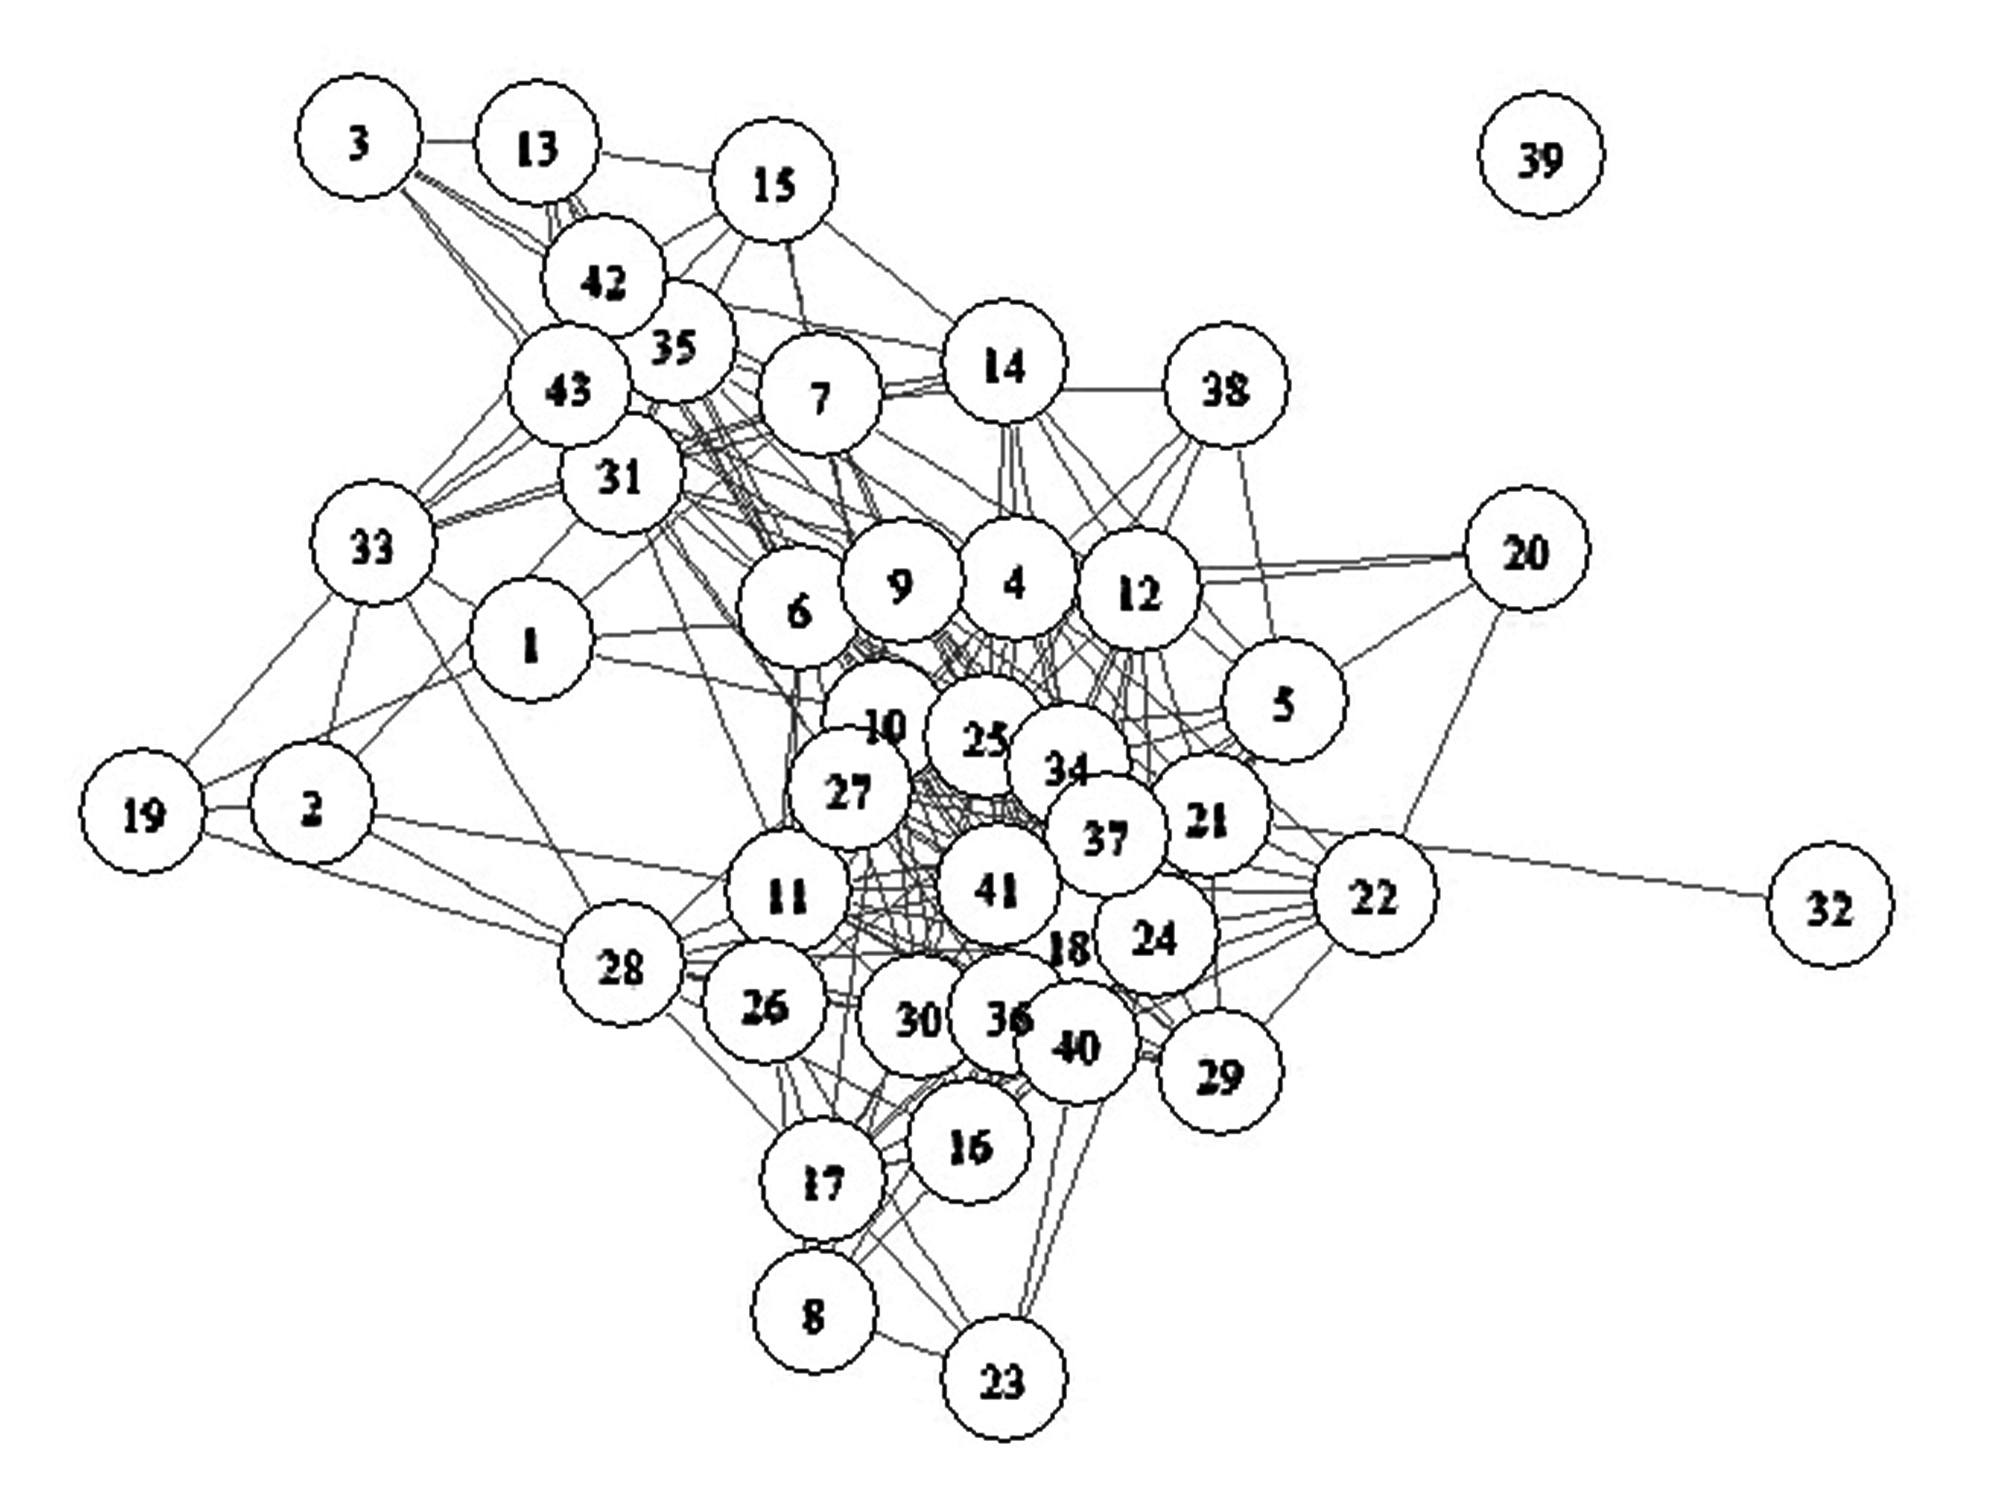
\includegraphics[width=0.6\linewidth]
		{ch-usage/figures/visgraph}
		\caption[Visual correlation graph output from the visualization 
		system.]{Visual correlation
			graph output from the visualization system.}
		\label{fig:usage:visg}
	\end{center}
\end{figure}
\bodyspacing

The final resulting visual correlation graph $\hat{G}$ is shown in 
Figure~\ref{fig:usage:visg}. Interestingly, only stock 39 (which corresponds to 
ticker TMO) has a degree of zero. This indicates 
that TMO is one of the best stocks to select because it is ``visually not 
correlated'' with any other stock and, by proxy, independent of all other 
stocks. Unsurprisingly, 
TMO does not show up in any of the top six ``visually correlated'' scatter 
plots depicted in Figure~\ref{fig:usage:interestingplots}. Stock 32 (which 
corresponds to ticker PRGO) has a degree of one and is the second-most 
``independent'' stock; as with TMO, PRGO is not a part of any of the top six 
most ``visually correlated'' scatter plots.

The visual graph has 252 edges, which makes it fairly sparse (there are a total 
of ${43\choose 2} = 903$ possible edges). Recall from 
Sections~\ref{sec:usage:stockselection} and~\ref{sec:usage:newanalysis} that we 
construct each numerical correlation graph $\hat{G}^{i,\text{num}}, i\in 
\{1,...,4\}$ with threshold $t = 0.15$ in order for the \textit{non-correlated} 
relations to be sparse; this makes the graphs $\hat{G}^{i,\text{num}}$ much 
more dense than $\hat{G}$. 
In order to more directly compare the visual and numerical graphs, we adjust 
the threshold value $t$ for each correlation metric such that each graph has 
about 250 edges. To be clear, these adjusted graphs are not used in the rest of 
the application; adjustment is for the purposes of examining the differences 
between $\hat{G}$ and $\hat{G}^{i,\text{num}}$ visually and better 
understanding the data. 
The adjusted Pearson's correlation graph uses a value of $t = 0.5$, the 
adjusted Spearman's correlation graph uses a value of $t = 0.49$, the adjusted 
Kendall's correlation graph uses a value of $t = 0.32$, and the adjusted 
distance correlation graph uses a value of $t = 0.28$. 
The resulting numerical correlation graphs are shown in 
Figure~\ref{fig:usage:numg}. By examining the 
threshold values alone, it is clear which graphs might be over-fitting the 
dependencies and, as such, require a higher threshold value in order to yield a 
sparser, more interpretable graph; thus, we can conjecture that the distance 
correlation graph is closest to the visual correlation graph. Interestingly, 
however, each adjusted numerical graph is able to capture the ``independence'' 
of TMO and PRGO. This suggests that the ``independence'' of these two stocks 
are truly robust; as such, we should expect the best-performing portfolios to 
include both TMO and PRGO.

\begin{figure}[htb]
	\begin{center}
		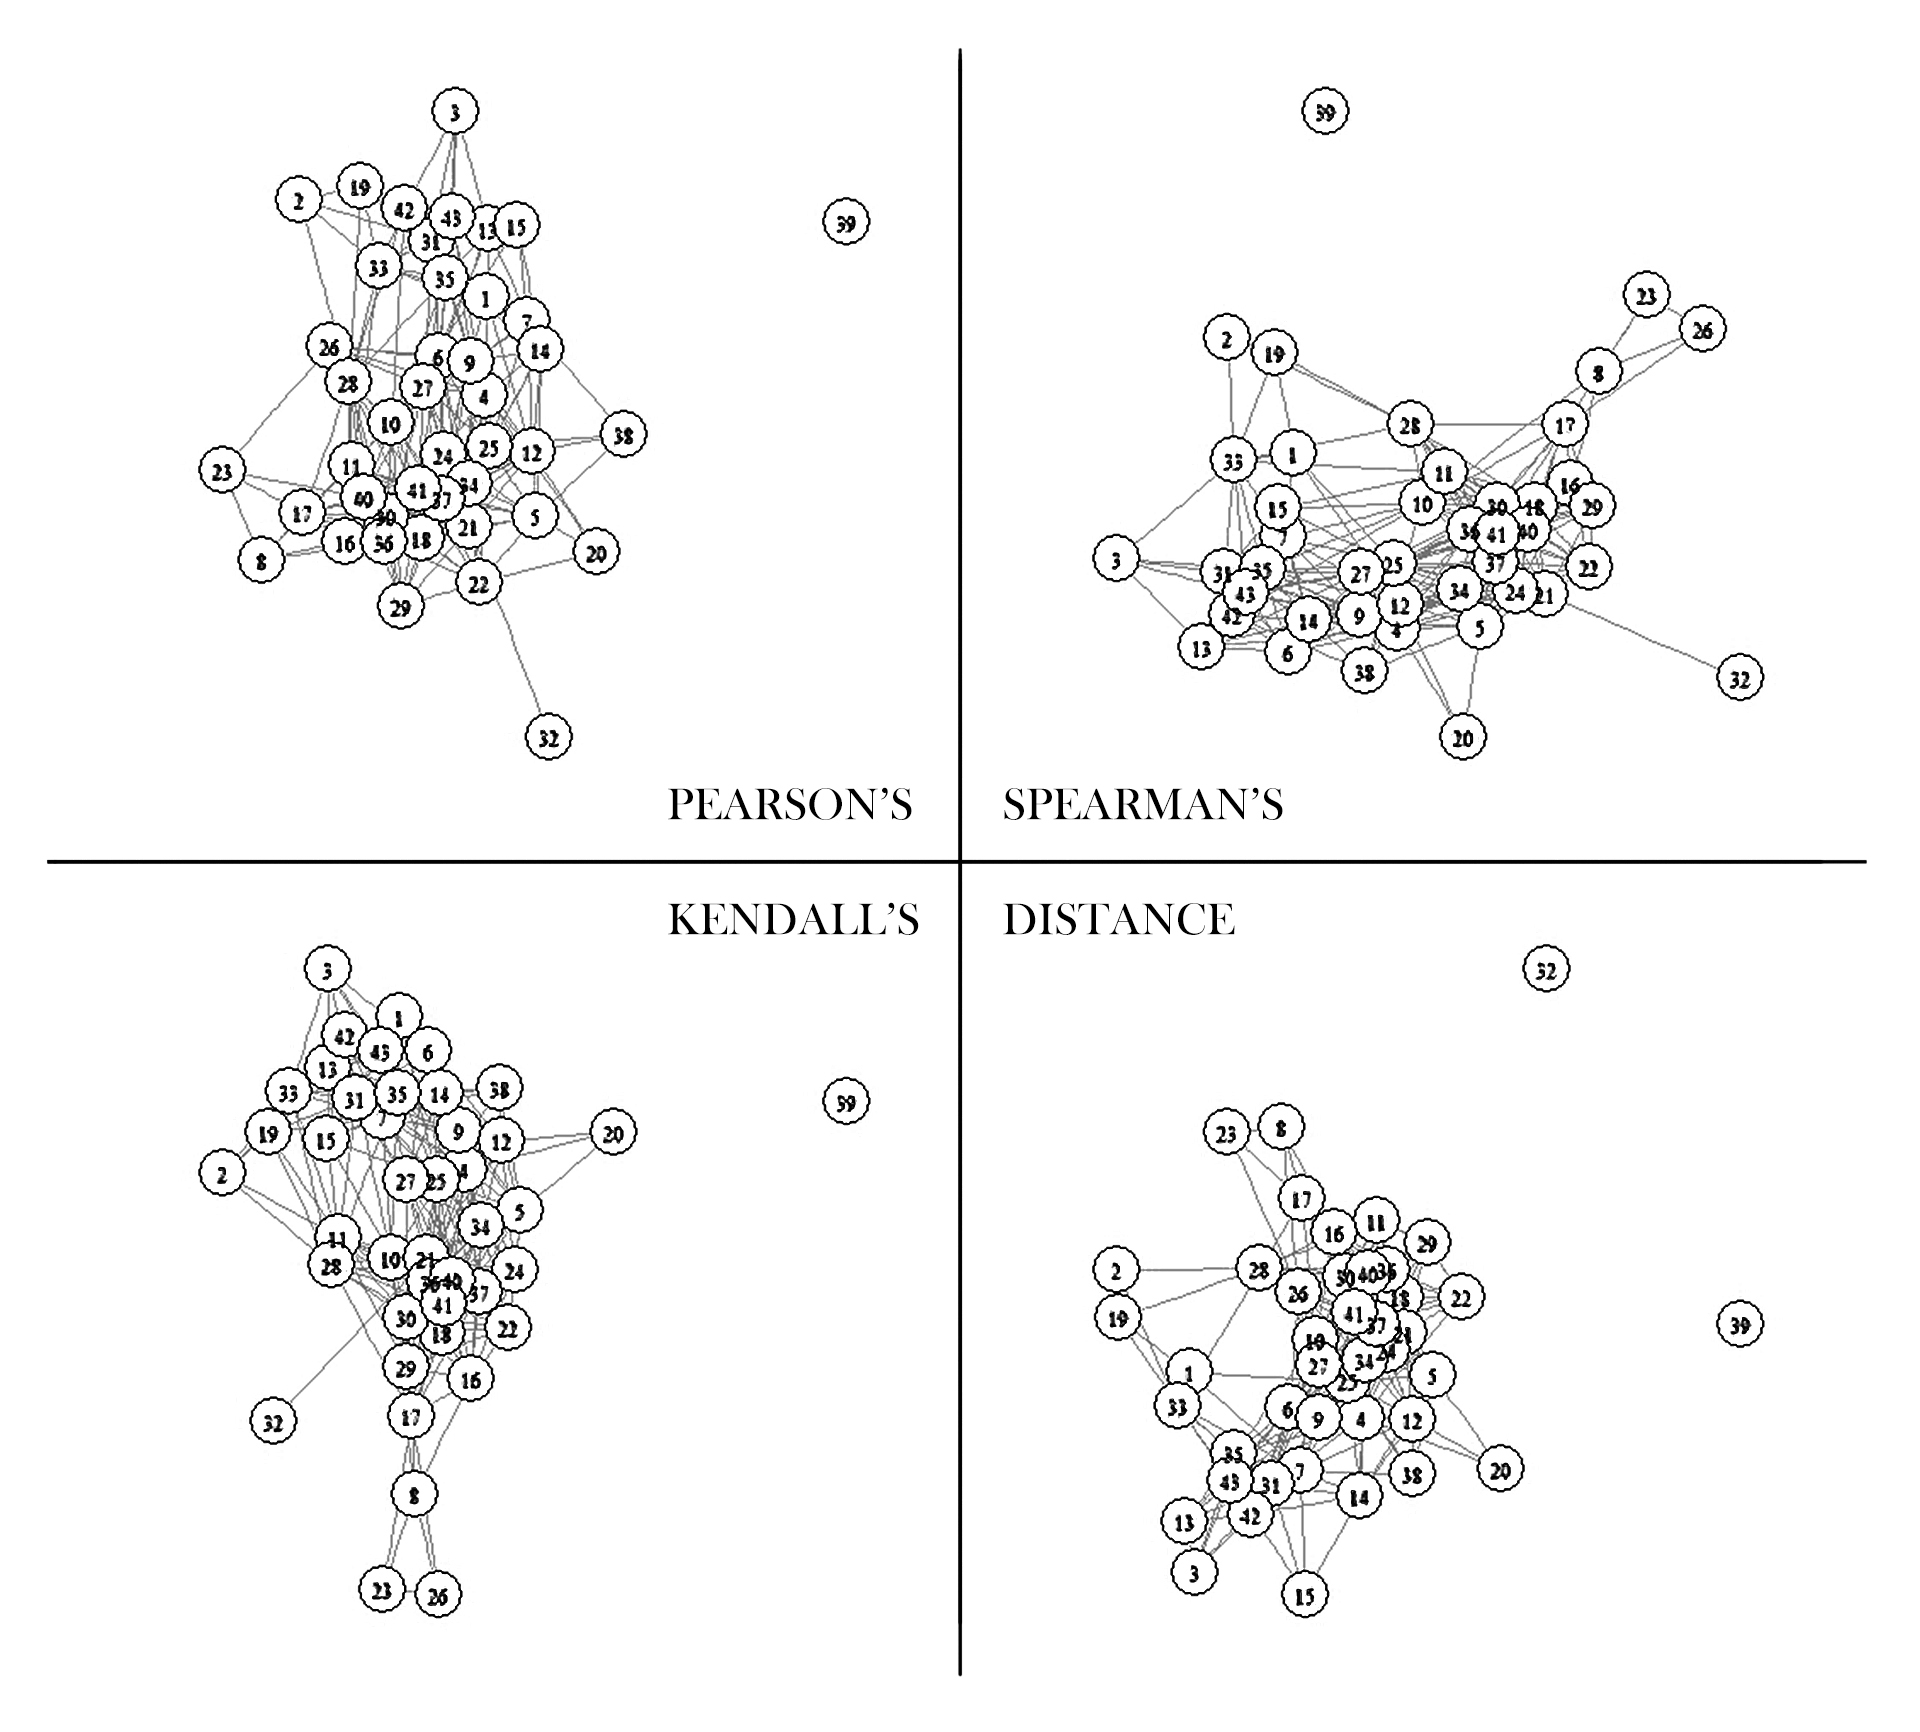
\includegraphics[width=1\linewidth]
		{ch-usage/figures/numgraphs}
		\caption[Numerical correlation graphs (sparse).]{Numerical correlation 
		graphs (sparse). \textit{Upper left:} Pearson's correlation graph with 
		threshold $t = 0.5$. \textit{Upper right:} Spearman's correlation graph 
		with threshold $t = 0.49$. \textit{Bottom left:} Kendall's correlation 
		graph with threshold $t = 0.32$. \textit{Bottom right:} Distance 
		correlation graph with threshold $t = 0.28$.}
		\label{fig:usage:numg}
	\end{center}
\end{figure}

\newpage
It turns out that the graph comparison procedure does determine that the 
\textbf{distance correlation graph} is closest to the visual correlation graph. 
Thus, $\hat{G}^* = \hat{G}^{4,\text{num}}$ (the index of 4 corresponds to the 
distance correlation graph). 
The computed graph differences may be found in Table~\ref{tab:usage:graphdiff}.
Then, each portfolio $P^i, i\in \{1,...,4\}$ is selected given its 
corresponding numerical correlation graph $\hat{G}^{i,\text{num}}$ where $P^* = 
P^4$ (again, these are not the adjusted numerical correlation graphs from 
earlier). The selection is performed using the procedure detailed in 
Section~\ref{sec:usage:stockselection}. Each portfolio's 
composition is summarized in Table~\ref{tab:usage:returns}. Only the Pearson's 
correlation portfolio and distance correlation portfolio include TMO, the most 
``visually not correlated'' stock. On the other hand, only the Spearman's 
correlation portfolio and distance correlation portfolio include 
PRGO, the second-most ``visually not correlated'' stock. This suggests that the 
distance correlation portfolio, which includes both, will perform the strongest.
The portfolio compositions reinforce the idea that the distance correlation 
graph is most similar to the visual correlation graph in this application, and 
the compositions also suggest that the other correlation coefficient metrics 
can still capture some component of the most ``visually not correlated'' stocks 
even as their density increases.

Finally, the ``buy and hold'' performance of yearly returns and cumulative 
sum of returns are plotted for the S\&P 500 (the control) and
all portfolios $P^i, i \in \{1,...,4\}$. The plots may be found in 
Figure~\ref{fig:usage:returns}, and the associated 
data may be found in Table~\ref{tab:usage:returns}. Note 
that the returns for 2006 and 2014 are low because the data begins 
on 3/14/2006 and ends on 5/13/2004; as such, the returns for 2006 and 2014 do 
not reflect a full year's worth of data. We focus mostly on the 
full years between 2006 and 2014, giving special attention to the portfolios' 
performance during the financial crisis. 

In line with expectations, the portfolio $P^*$, which was constructed from the 
numerical correlation graph $\hat{G}^* = \hat{G}^{4,\text{num}}$ (distance 
correlation) most similar to the visual correlation graph $\hat{G}$, 
performs the strongest by far. $P^*$ consistently posts the highest returns 
year after year. Though it doesn't seem to strongly outperform on a yearly 
basis, the differences really add up; this can clearly be seen in the 
cumulative sum of yearly returns. Further 
consider the financial crisis; $P^*$ has the least negative returns of 2008. 
This indicates that the VS is doing a good job capturing our intuition 
regarding the dependencies among various stocks, which translates into the 
visual graph $\hat{G}$, the selection of $\hat{G}^*$, and the subsequent 
selection of $P^*$, 
a portfolio that is well-balanced and captures the spirit of the ``buy and 
hold'' model described in Section~\ref{sec:intro:finance}.
Both the Pearson's correlation portfolio (which included TMO but not PRGO) and 
the Spearman's correlation portfolio (which included PRGO but not TMO) 
performed rather average. What is interesting to observe, however, is their 
relative performance. Although TMO is supposedly more 
``visually not correlated'' and should thereby be a better pick than PRGO, the 
Pearson's correlation portfolio underperforms Spearman's until around 2012. It 
is difficult to make any concrete conclusions about which is better, however, 
since each portfolio contains 4 other stocks that we have not examined 
in-depth up to this point; a cursory examination of the corresponding 
portfolios yields the fact that they both contain SYK and VAR.
As noted earlier in Section~\ref{sec:usage:stockselection}, the proposed stock 
selection strategy is simple, but every selected portfolio has outperformed the 
S\&P 500, suggesting that a more sophisticated selection procedure would 
yield even more fruitful returns.

\subsection{Extensions}
\label{sec:usage:extensions}

It should also be noted that, while a rebalancing method performs better in 
practice~\cite{liuh2016}, the ``buy and hold'' strategy is better-suited for 
observing portfolio performances over time with less external influences, 
providing a more concrete basis of comparison for the performance of 
$\hat{G}^*$. 
Actually, the procedure described in Section~\ref{sec:usage:newanalysis}
can certainly be repeated yearly (once a year's worth of new data has been 
collected) to determine the direction in which to 
rebalance the portfolio. However, the procedure should be modified to take 
transaction costs into account. Another extension stems from the idea that the 
portfolio weights of each stock can certainly be optimized; currently, each 
stock holds equal weight within its portfolio. These extensions may improve 
upon portfolio management techniques that this application does not utilize.

%$P^{\text{vis}}$ catches up after a mediocre beginning, and there are other 
%interesting things to note about its performance that makes it difficult to 
%definitively say which portfolio is ``better''. Consider the financial crisis; 
%while the positive returns and recovery of $P^{\text{vis}}$ are muted, it has 
%the most significant least negative returns of 2008. This is an indication
%that the visual graph is capturing precisely what we wish for it to capture 
%(independence and dependence among various stocks), which is translating into 
%a portfolio that is well balanced and captures the spirit of the ``buy and 
%hold'' model described in Section~\ref{sec:intro:finance}. The persistence in 
%holding the portfolio ends up paying off returns rapid increase until the 
%portfolio is the top performer in 2011 and beyond.

\begin{landscape}
	\tablespacing
	\begin{longtable}{p{0.1\linewidth}p{0.15\linewidth}p{0.13\linewidth}
			p{0.13\linewidth}p{0.13\linewidth}p{0.13\linewidth} }
		
		% First page heading
		\caption[Computed differences between visual and numerical correlation 
		graphs.]{Computed differences between visual and numerical correlation 
		graphs. See Section~\ref{sec:gc:methods} for details on each graph 
		summarization metric. (*) indicates the numerical correlation graph 
		most similar to visual correlation graph.} 
		\label{tab:usage:graphdiff}\\
		\toprule
		\textbf{Graph Type} & \textbf{Centrality \newline (degree)} & 
		\textbf{Centrality \newline (closeness)} & 
		\textbf{Centrality \newline (betweenness)} & 
		\textbf{Assortativity} & \textbf{Distance \newline matrix} \\
		\midrule
		\endfirsthead
		
		% Last page footer
		\bottomrule
		\endlastfoot

		Pearson's & 0.0034 & 0.0119 & 0.0032 & 0.061 & 0.0313\\
		
		Spearman's & 0.0052 & 0.0079 & 0.0032 & 0.0773 & 0.029\\
		
		Kendall's & 0.0002 & 0.019 & 0.0024 & 0.0559 & 0.0253\\
		
		Distance (*) & 0.0018 & 0.0276 & 0.0012 & 0.0465 & 0.0206\\
		
		\midrule
		
		& \textbf{Community\newline (random walk)} & 
		\textbf{Community \newline (infomap)} & 
		\textbf{Community \newline (betweenness)} & 
		\textbf{Edge\newline connectivity} & 
		\textbf{Edge density \newline histogram} \\
		 	
		\midrule
		
		Pearson's & 0.7602 & 0.5039 & 0.6488 & 1 & 0.6014\\
		
		Spearman's & 0.8478 & 0.5039 & 0.6948 & 1 & 0.5625\\
		
		Kendall's & 1 & 0.5039 & 0.7284 & 1 & 0.4413\\
		
		Distance (*) & 0.253 & 0.5039 & 0.5437 & 1 & 0.2455\\
		
	\end{longtable}
	\bodyspacing
\end{landscape}





\begin{figure}[htb]
	\begin{center}
		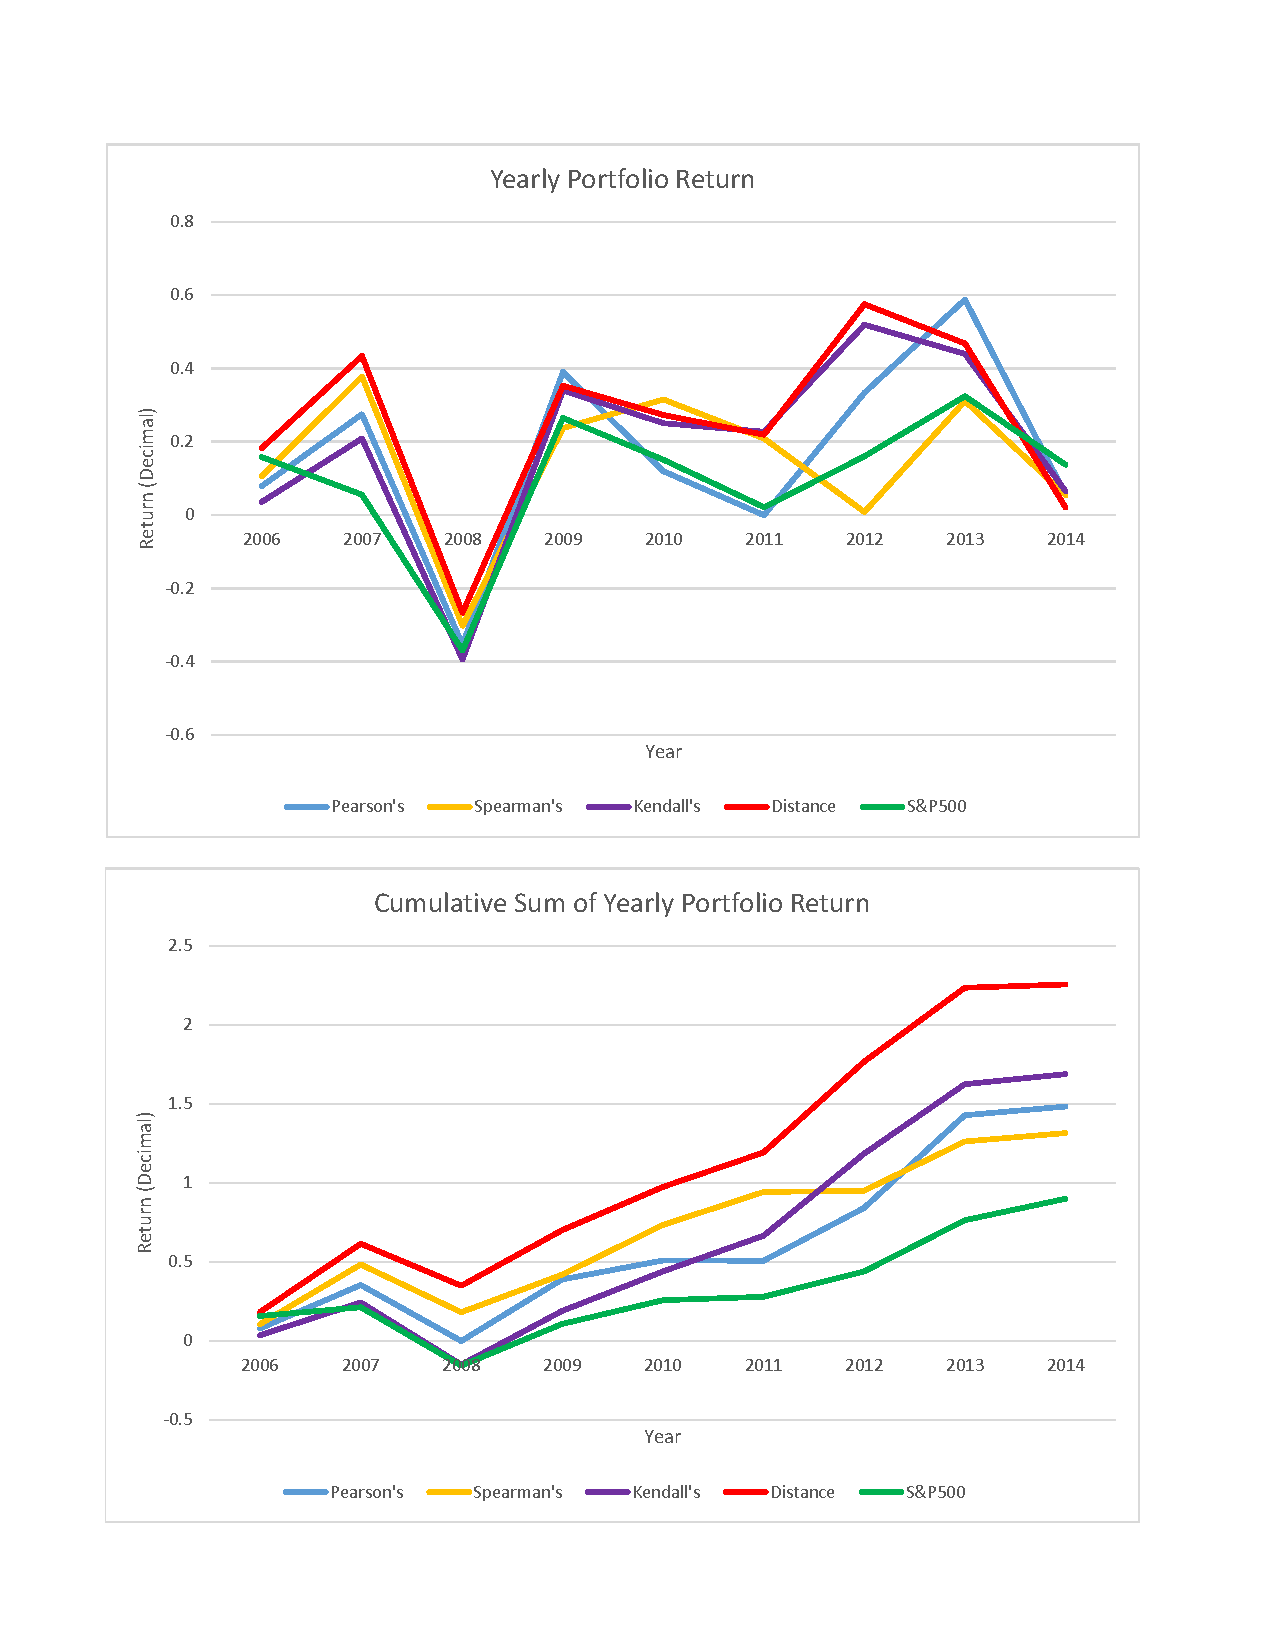
\includegraphics[width=1\linewidth]
		{ch-usage/figures/Results_YearlyReturns.pdf}
		\caption[Yearly and cumulative performance of the selected portfolios 
		and the S\&P 500.]{Yearly and cumulative performance of the selected 
		portfolios and the S\&P 500. Note that the ``yearly'' returns for 2006 
		and 2014 are low because the data begins on 3/14/2006 and ends on 
		5/13/2004; as such, those returns do not reflect a full year of data. 
		The associated data may be found in Table~\ref{tab:usage:returns}.}
		\label{fig:usage:returns}
	\end{center}
\end{figure}




\begin{landscape}
\tablespacing
\begin{longtable}{p{0.15\linewidth}p{0.15\linewidth}p{0.05\linewidth}
p{0.05\linewidth}p{0.05\linewidth}p{0.05\linewidth} 
p{0.05\linewidth}p{0.05\linewidth}p{0.05\linewidth} 
p{0.05\linewidth}p{0.05\linewidth}p{0.05\linewidth} 
p{0.05\linewidth}}
	
	% First page heading
	\caption[Yearly returns of the portfolios selected from the numerical 
	correlation graphs.]{Yearly returns (in decimal) of the portfolios selected 
	from the numerical correlation graphs.  (*) indicates the numerical 
	correlation graph most similar to visual correlation graph.} 
	\label{tab:usage:returns}\\
	\toprule
	\textbf{Graph Type} & \textbf{Portfolio} & \textbf{2006} 
	& \textbf{2007} & \textbf{2008} & \textbf{2009} & 
	\textbf{2010} & \textbf{2011} & \textbf{2012} & 
	\textbf{2013} & \textbf{2014} \\
	\midrule
	\endfirsthead
	
	% Future page heading
	\caption[]{(continued)}\\
	\toprule
	\textbf{Graph Type} & \textbf{Portfolio} & \textbf{2006} 
	& \textbf{2007} & \textbf{2008} & \textbf{2009} & 
	\textbf{2010} & \textbf{2011} & \textbf{2012} & 
	\textbf{2013} & \textbf{2014} \\
	\midrule
	\endhead
	
	% Page footer
	\midrule
	\multicolumn{11}{r}{(Continued on next page)}\\
	\endfoot
	
	% Last page footer
	\bottomrule
	\endlastfoot

	S\&P 500 \newline (CONTROL) & \textbf{Total} & 
	0.158&0.055&-0.37&0.265&0.151&0.021&0.16&0.324&0.137\\
	
	\cmidrule[0.1pt](l{0.5em}r{0.5em}){1-11}	
	
	Pearson's &CI&0.041&0.226&-0.686&1.099&0.041&0.147&0.274&0.637&0.011\\
	&GILD&0.056&0.417&0.111&-0.154&-0.162&0.129&0.795&1.045&0.069\\
	&SYK&0.15&0.362&-0.46&0.267&0.079&-0.061&0.121&0.393&0.073\\
	&TMO&0.276&0.274&-0.409&0.4&0.161&-0.188&0.432&0.758&0.057\\
	&VAR&-0.131&0.096&-0.328&0.337&0.479&-0.031&0.046&0.106&0.064\\
	&\textbf{Total}&0.078&0.275&-0.354&0.39&0.119&-0.001&0.333&0.588&0.055\\
	
	\cmidrule[0.1pt](l{0.5em}r{0.5em}){1-11}	
	
	Spearman's &HUM&0.122&0.362&-0.505&0.177&0.247&0.615&-0.206&0.523&0.184\\
	&LH&0.291&0.028&-0.147&0.162&0.175&-0.022&0.008&0.055&0.092\\
	&PRGO&0.096&1.041&-0.072&0.243&0.597&0.542&0.073&0.479&-0.144\\
	&SYK&0.15&0.362&-0.46&0.267&0.079&-0.061&0.121&0.393&0.073\\
	&VAR&-0.131&0.096&-0.328&0.337&0.479&-0.031&0.046&0.106&0.064\\
	&\textbf{Total}&0.106&0.378&-0.302&0.237&0.315&0.208&0.008&0.311&0.054\\
	
	\cmidrule[0.1pt](l{0.5em}r{0.5em}){1-11}	
	
	Kendall's&MCK&-0.039&0.297&-0.404&0.63&0.138&0.118&0.256&0.676&0.117\\
	&REGN&0.231&0.203&-0.24&0.317&0.358&0.688&2.086&0.609&0.03\\
	&SYK&0.15&0.362&-0.46&0.267&0.079&-0.061&0.121&0.393&0.073\\
	&UNH&-0.035&0.084&-0.543&0.148&0.199&0.422&0.086&0.41&0.04\\
	&VAR&-0.131&0.096&-0.328&0.337&0.479&-0.031&0.046&0.106&0.064\\
	&\textbf{Total}&0.035&0.209&-0.395&0.34&0.25&0.227&0.519&0.439&0.065\\
	
	%\cmidrule[0.1pt](l{0.5em}r{0.5em}){1-11}			
	\newpage
	
	Distance (*)&JNJ&0.137&0.036&-0.078&0.113&-0.006&0.099&0.108&0.346&0.111\\
	&PRGO&0.096&1.041&-0.072&0.243&0.597&0.542&0.073&0.479&-0.144\\
	&REGN&0.231&0.203&-0.24&0.317&0.358&0.688&2.086&0.609&0.03\\
	&TMO&0.276&0.274&-0.409&0.4&0.161&-0.188&0.432&0.758&0.057\\
	&WAT&0.169&0.615&-0.536&0.691&0.254&-0.047&0.177&0.148&0.048\\
	&\textbf{Total}&0.182&0.434&-0.267&0.353&0.273&0.219&0.575&0.468&0.021\\
	
\end{longtable}
\bodyspacing
\end{landscape}